\documentclass[11pt]{article}

\usepackage[a4paper,margin=2.35cm]{geometry}
\usepackage[T1]{fontenc}
\usepackage[utf8]{inputenc}
\usepackage{lmodern}
\usepackage{microtype}
\usepackage{amsmath,amssymb}
\usepackage{booktabs}
\usepackage{enumitem}
\usepackage{listings}
\usepackage{tikz}
\usepackage{hyperref}
\usepackage{xcolor}
\usetikzlibrary{arrows.meta,positioning,fit}

\hypersetup{
  pdftitle={Walrus Memory Graphs: Bitemporal Hypertext for Persistent AI Agents on Sui and Walrus},
  pdfauthor={Daniel Devatman Hromada},
  colorlinks=true,
  linkcolor=black,
  citecolor=black,
  urlcolor=black
}

\lstset{
  basicstyle=\ttfamily\small,
  breaklines=true,
  frame=single,
  columns=fullflexible,
  showstringspaces=false
}

\title{\textbf{Walrus Memory Graphs: Bitemporal Hypertext for Persistent AI Agents on Sui and Walrus}\\
\large Typed \texttt{wal://} Links Between Evolving Social Entities and Immutable Episodes}
\author{Daniel Devatman Hromada\\\small Universit\"at der K\"unste Berlin}
\date{Version 2 --- October 2026}

\begin{document}
\maketitle

\begin{abstract}
Contemporary conversational agents usually treat memory as a collection of text fragments or vectors retrieved by semantic similarity. This is useful for recall, but it poorly represents identity, temporal evolution, provenance, and relationships among memories. We propose the \emph{Walrus Memory Graph}: a persistent, typed, hypertext-like memory architecture that combines mutable Sui objects with immutable Walrus blobs. Stable social entities---initially persons and Matrix rooms---receive persistent Sui object identifiers. Their changing descriptions are stored as append-only Walrus revisions, with the Sui object pointing to the current head. Episodic memories are immutable Walrus documents encoding what happened, when and where it happened, and who participated. Episodes refer to persons and rooms through an application-level URI scheme such as \texttt{wal://person/<sui-object-id>} and \texttt{wal://room/<sui-object-id>}. Each episode may additionally pin the exact interpersonal-memory revision that was current when the episode occurred. This produces a bitemporal graph in which an agent can ask both ``what do I know about this person now?'' and ``what did I know about this person when this event occurred?'' The design preserves historical lineage, supports cryptographic verification of stored states, and can keep sensitive social structure encrypted. We describe the data model, resolution semantics, update protocol, privacy model, concurrency rules, and a Matrix-native reference implementation suitable for persistent multi-user AI agents.

\smallskip
\noindent\emph{Version 2} reports on that implementation, \emph{Walden3}, deployed since 24~September~2026 in four Matrix rooms on three homeservers and running entirely on a local open-weight model (IBM Granite~4.0 H-Small via Ollama). Its interpersonal memory is a set of facts with provenance---who said it, when, in which room and episode---scoped to the room where it was learned; each room's memory is mirrored to Walrus Memory on Sui mainnet as an encrypted, hash-chained, verifiable checkpoint that can be loaded and synchronised into other rooms; whole rooms can be archived with explicit per-person consent. With memory, the agent answers questions about its interlocutors correctly that it otherwise answers by invention. We report the four tests proposed in version~1, costs, latencies, and the failure modes of memory extraction with a small model, together with the deterministic guards that fixed them.
\end{abstract}

\section{Introduction}

Long-lived AI agents need more than retrieval. They need a notion of \emph{continuing identity}: the ability to recognize that a human encountered today is the same human encountered months earlier, that a conversational room has accumulated its own culture and history, and that an event belongs to a particular moment in the evolving relationship among these entities.

Most current agent-memory systems reduce this problem to a searchable store of textual memories or embedding vectors. Such systems can retrieve relevant fragments, but they make several important questions awkward:

\begin{itemize}[nosep]
    \item Which memories describe the same persistent person or social space?
    \item How did the agent's understanding of that person change over time?
    \item Which exact version of a person's memory informed an action in a past episode?
    \item Can old memories remain verifiable rather than being silently overwritten?
    \item Can an episode link directly to the people and rooms involved, as a hypertext document links to other documents?
\end{itemize}

This paper proposes a simple answer based on the complementary semantics of Sui and Walrus. Sui objects provide persistent identity: an object's contents may evolve while its object ID remains stable~\cite{sui}. Walrus provides immutable content-addressed storage: changed stored bytes produce a new blob identifier, leaving the previous version independently addressable~\cite{walrus-lineage,walrus-whitepaper}. The combination yields a natural division of labor:

\begin{quote}
\textbf{Sui represents what persists. Walrus represents what happened to be true at a particular revision.}
\end{quote}

We call the resulting structure a \emph{Walrus Memory Graph}. It borrows from the original hypertext idea of traversable associative structures~\cite{bush,nelson}, from episodic-memory theory~\cite{tulving}, and from recent agent architectures that treat memory as a first-class component~\cite{generative-agents,memgpt}. Unlike a conventional knowledge graph, however, the proposed graph explicitly combines mutable identity nodes with immutable historical states.

The motivating implementation is a Matrix-native conversational agent, here called \emph{Walden}. Matrix is useful because users, rooms and events already possess protocol-level identifiers~\cite{matrix-spec}. Nevertheless, the architecture is not Matrix-specific: Matrix supplies the social substrate, while Sui and Walrus supply the persistent memory substrate.

The contribution is therefore not merely ``put chatbot memories on decentralized storage.'' The contribution is a typed, temporal addressing model in which memory becomes navigable hypertext.

\section{Design Principles}

The architecture follows six principles.

\paragraph{Persistent identity.}
A person or social room should keep the same logical identity even when the agent's beliefs about it change. We therefore assign each such entity a stable Sui object.

\paragraph{Immutable historical state.}
A past description should never be overwritten. Every revision is stored as a new Walrus blob. Walrus blob IDs act as immutable handles to stored bytes~\cite{walrus-lineage}.

\paragraph{Typed references.}
Memories should refer to one another explicitly rather than only by semantic similarity. We define a small \texttt{wal://} namespace for persons, rooms, episodes and raw blobs.

\paragraph{Dual temporal access.}
The graph should support both current-state queries and historical-state queries. A stable person reference resolves to the current head, while a pinned blob reference resolves to the exact historical revision.

\paragraph{Privacy by encryption.}
Walrus blobs are publicly retrievable when their blob IDs are known unless the application encrypts them. Sensitive memories must therefore be encrypted before storage; Walrus Memory supports Seal-based encryption~\cite{walrus-agent-loop,walrus-console}.

\paragraph{Sparse use of on-chain state.}
Not every memory requires a Sui object. Stable entities receive Sui identities; high-volume episodic records remain inexpensive immutable Walrus blobs. This keeps the chain as an identity and head-pointer layer rather than a transcript database.

\section{Memory Types}

We initially distinguish three memory types.

\subsection{Interpersonal memory: who}

An \emph{interpersonal memory} represents the agent's evolving model of a human counterpart. It may contain stable facts, preferences, shared history, projects, unresolved topics, confidence values and provenance links. It is not the human being itself; it is explicitly the agent's current memory \emph{of} that human.

For each known person $p$, the system creates a Sui object $O_p$ with stable identifier $id(O_p)$. The object's principal mutable field is a head pointer

\[
H(O_p) = b_k,
\]

where $b_k$ is the Walrus blob ID of the latest interpersonal-memory revision.

Each revision contains a link to its predecessor:

\[
P(b_k)=b_{k-1}, \qquad P(b_0)=\bot.
\]

Thus the current Sui object identifies the latest state, while repeated application of $P$ reconstructs the complete retained lineage.

\subsection{Room memory: social context}

A Matrix room is more than a bag of messages. Long-running rooms accumulate topics, norms, roles, recurring projects, inside references, shared decisions and characteristic interaction patterns. We therefore introduce a second persistent entity type: \emph{room memory}.

A Matrix room known to the agent receives a stable Sui object $O_r$. Its current Walrus head contains the agent's evolving model of that room. The public Sui object need not contain the literal Matrix room ID. The binding between a Matrix room ID and its Sui memory object can remain local or encrypted.

Room memory may include references to interpersonal memories, for example the recurrent participants of the room:

\begin{lstlisting}
{
  "schema": "walden-room-memory/1",
  "previous": "wal://blob/<previous-room-memory-blob>",
  "topic": "...",
  "shared_context": ["..."],
  "norms": ["..."],
  "participants": [
    "wal://person/0x...",
    "wal://person/0x..."
  ],
  "open_threads": ["..."]
}
\end{lstlisting}

\subsection{Episodic memory: what, where and when}

An \emph{episodic memory} represents an event situated in time and context. In the spirit of Tulving's distinction between episodic and semantic memory~\cite{tulving}, an episode is not primarily a timeless fact. It records that something happened.

A minimal episode answers:

\begin{center}
\textbf{what happened? \quad when? \quad where/in which room? \quad who was involved?}
\end{center}

Episodes are high-volume and naturally append-only, so the default representation is a Walrus blob rather than a Sui object. An episode can directly reference the stable persons and rooms involved.

\begin{lstlisting}
{
  "schema": "walden-episode/1",
  "when": {
    "start": "2026-09-22T11:14:00+02:00",
    "end":   "2026-09-22T12:03:00+02:00"
  },
  "room": "wal://room/0x...",
  "where": {
    "kind": "virtual",
    "label": "Matrix conversation"
  },
  "what": {
    "type": "conversation",
    "summary": "Discussion of persistent agent memory graphs"
  },
  "who": [
    {
      "person": "wal://person/0x...",
      "memory_at_time": "wal://blob/<person-revision-A>"
    },
    {
      "person": "wal://person/0x...",
      "memory_at_time": "wal://blob/<person-revision-B>"
    }
  ],
  "related": []
}
\end{lstlisting}

The paired fields \texttt{person} and \texttt{memory\_at\_time} are central to the design. The first identifies the person diachronically. The second freezes the agent's knowledge of that person at the moment of the episode.

\section{The \texttt{wal://} Hypertext Namespace}

We define an application-level URI convention:

\begin{lstlisting}
wal://person/<sui-object-id>
wal://room/<sui-object-id>
wal://episode/<walrus-blob-id>
wal://blob/<walrus-blob-id>
\end{lstlisting}

This is a Walden/Walrus-Memory-Graph convention, not an official Walrus URI scheme. Its purpose is to give stored memories typed, traversable references. The type component determines how the identifier is resolved.

\begin{table}[h]
\centering
\caption{Resolution semantics of the proposed \texttt{wal://} namespace.}
\begin{tabular}{lll}
\toprule
Type & Identifier & Resolution \\
\midrule
\texttt{person} & Sui object ID & read Sui object $\rightarrow$ current Walrus head \\
\texttt{room} & Sui object ID & read Sui object $\rightarrow$ current Walrus head \\
\texttt{episode} & Walrus blob ID & retrieve immutable episode blob \\
\texttt{blob} & Walrus blob ID & retrieve exact immutable blob \\
\bottomrule
\end{tabular}
\end{table}

The namespace deliberately mixes two kinds of identifiers, but never ambiguously: the URI type tells the resolver whether the following identifier belongs to Sui or Walrus.

For a stable entity $x$, current-state resolution is

\[
R_t(\texttt{wal://person/}x)=\operatorname{WalrusGet}(H_t(x)).
\]

By contrast,

\[
R(\texttt{wal://blob/}b)=\operatorname{WalrusGet}(b)
\]

is temporally invariant for as long as the blob remains retained and retrievable.

\section{A Bitemporal Memory Graph}

The combination of stable references and pinned historical references creates a useful form of bitemporality.

Consider an episode $e$ involving Alice. The episode stores both

\begin{lstlisting}
"person": "wal://person/<alice-sui-id>"
\end{lstlisting}

and

\begin{lstlisting}
"memory_at_time": "wal://blob/<alice-v4>"
\end{lstlisting}

Months later, Alice's Sui person object may point to revision $v_{17}$. The same old episode can now answer two distinct queries:

\begin{description}[style=nextline]
\item[What does the agent know about Alice now?]
Resolve \texttt{wal://person/<alice-sui-id>} through the current Sui head.

\item[What did the agent know about Alice during this episode?]
Resolve the pinned \texttt{wal://blob/<alice-v4>} reference.
\end{description}

This distinction matters because agent memory is epistemic, not merely archival. A later correction should change present belief without rewriting what the agent actually believed in the past.

Formally, let $E$ be the set of stable entities, $B$ the set of immutable Walrus revisions, and $Q$ the set of episodes. At time $t$ the memory graph is

\[
G_t=(V,\mathcal{E}_t), \qquad V=E\cup B\cup Q.
\]

Important edge types include:

\begin{align*}
\textsf{head}_t &: E \rightarrow B,\\
\textsf{previous} &: B \rightarrow B\cup\{\bot\},\\
\textsf{participant} &: Q \rightarrow E,\\
\textsf{snapshot} &: Q \rightarrow B,\\
\textsf{room} &: Q \rightarrow E,\\
\textsf{related} &: Q \rightarrow Q\cup B.
\end{align*}

Only \textsf{head} is intrinsically mutable. The remaining historical edges are append-only once written.

\section{Architecture}

Figure~\ref{fig:graph} shows a minimal graph with two people, one Matrix room and one episode.

\begin{figure}[h]
\centering
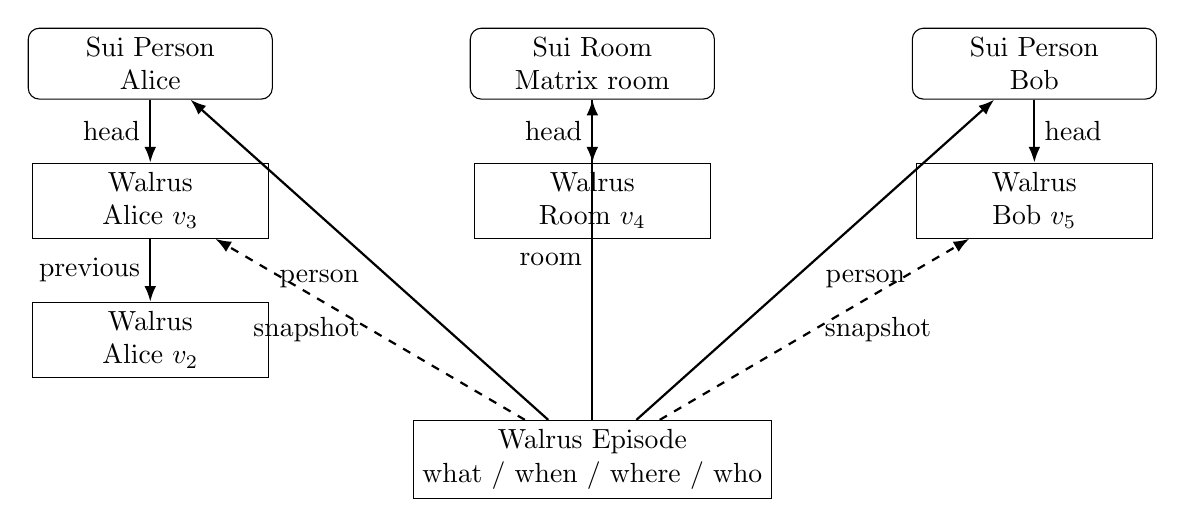
\begin{tikzpicture}[
    node distance=8mm and 14mm,
    sui/.style={draw,rounded corners,align=center,minimum width=31mm,minimum height=9mm},
    wal/.style={draw,align=center,minimum width=30mm,minimum height=9mm},
    arr/.style={-{Latex[length=2mm]},thick}
]
\node[sui] (alice) {Sui Person\\Alice};
\node[wal,below=of alice] (a3) {Walrus\\Alice $v_3$};
\node[wal,below=of a3] (a2) {Walrus\\Alice $v_2$};

\node[sui,right=25mm of alice] (room) {Sui Room\\Matrix room};
\node[wal,below=of room] (r4) {Walrus\\Room $v_4$};

\node[sui,right=25mm of room] (bob) {Sui Person\\Bob};
\node[wal,below=of bob] (b5) {Walrus\\Bob $v_5$};

\node[wal,below=23mm of r4] (ep) {Walrus Episode\\what / when / where / who};

\draw[arr] (alice) -- node[left]{head} (a3);
\draw[arr] (a3) -- node[left]{previous} (a2);
\draw[arr] (room) -- node[left]{head} (r4);
\draw[arr] (bob) -- node[right]{head} (b5);
\draw[arr] (ep) -- node[below left]{person} (alice);
\draw[arr] (ep) -- node[left]{room} (room);
\draw[arr] (ep) -- node[below right]{person} (bob);
\draw[arr,dashed] (ep) -- node[left]{snapshot} (a3);
\draw[arr,dashed] (ep) -- node[right]{snapshot} (b5);
\end{tikzpicture}
\caption{A Walrus Memory Graph combines stable Sui entity identities with immutable Walrus state and episode nodes. Solid entity-head edges resolve current state; pinned snapshot edges preserve historical epistemic state.}
\label{fig:graph}
\end{figure}

This architecture has an intentionally asymmetric topology. Persons and rooms are \emph{entities}; episodes are \emph{occurrences}. Entities need stable identity and mutable heads. Occurrences normally need only immutable storage.

\section{Update Protocol}

\subsection{First encounter}

When the agent encounters a previously unknown Matrix user, it performs the following conceptual procedure:

\begin{enumerate}[nosep]
    \item Create an initial encrypted interpersonal-memory document $m_0$ with \texttt{previous = null}.
    \item Store $m_0$ on Walrus and obtain blob ID $b_0$.
    \item Create a Sui person-memory object whose head equals $b_0$.
    \item Store the Matrix-user-ID $\leftrightarrow$ Sui-object-ID binding in a private local or encrypted identity index.
\end{enumerate}

The public Sui object therefore need not reveal the Matrix identifier.

\subsection{Interpersonal-memory revision}

Suppose the current head of person object $O_p$ is $b_k$. To incorporate new information:

\begin{enumerate}[nosep]
    \item Retrieve and decrypt $b_k$.
    \item Derive the new memory state $m_{k+1}$.
    \item Set \texttt{previous = wal://blob/$b_k$}.
    \item Encrypt and store $m_{k+1}$ on Walrus, yielding $b_{k+1}$.
    \item Atomically change $H(O_p)$ from $b_k$ to $b_{k+1}$.
\end{enumerate}

The old revision remains addressable and can be reached by following \texttt{previous} links.

\subsection{Optimistic concurrency}

A social agent may operate in several Matrix rooms simultaneously. Two workers could therefore read the same head and attempt concurrent updates. The Move update function should include an expected-parent guard:

\begin{lstlisting}
update_head(person_object,
            expected_head = old_blob_id,
            new_head      = new_blob_id)
\end{lstlisting}

The transaction succeeds only if the current head still equals \texttt{expected\_head}. Otherwise the worker reloads the newer state and rebases or merges its proposed update. This prevents a last-writer-wins race from silently deleting memory.

\subsection{Episode creation}

For each meaningful episode, the agent resolves every participant's current person head and the room's current head. The episode stores stable references and, where useful, pinned revision references. The episode is then encrypted and written as a new Walrus blob.

Crucially, an episode does not have to cause a new interpersonal revision. Observation and consolidation are separate operations. A high-volume conversation can therefore produce many episodes while interpersonal state is updated only when a durable fact, preference or relationship-level interpretation changes.

\section{Memory as Hypertext}

The architecture revives a central idea from early hypertext: information is useful not only because it can be searched, but because it can be \emph{traversed} through meaningful links~\cite{bush,nelson}. Vector retrieval and graph traversal solve different problems.

A semantic query such as ``what did Alice say about sustainable AI?'' may begin with vector recall. Once an episode is found, however, typed links provide deterministic navigation:

\[
\text{episode}
\rightarrow \text{person}
\rightarrow \text{current interpersonal head}
\rightarrow \text{previous revisions}.
\]

Or:

\[
\text{episode}
\rightarrow \text{room}
\rightarrow \text{current room memory}
\rightarrow \text{participants}.
\]

The graph therefore complements embeddings rather than replacing them. Embeddings answer \emph{which memory may be relevant?}; typed links answer \emph{what exactly is this memory connected to?}

This distinction is especially important for agentic behavior. An agent can use semantic recall to discover a relevant episode, then traverse explicit links to gather the people, room context and historically appropriate memory snapshots needed to interpret it.

\section{Epistemic Provenance}

A memory system should distinguish observations from inferences. Interpersonal memory can represent claims as structured assertions rather than unqualified prose:

\begin{lstlisting}
{
  "claim": "prefers concise technical explanations",
  "confidence": 0.86,
  "status": "active",
  "first_seen": "wal://episode/<...>",
  "last_confirmed": "wal://episode/<...>",
  "sources": [
    "wal://episode/<...>",
    "wal://episode/<...>"
  ]
}
\end{lstlisting}

This turns the memory graph into an epistemic graph: durable beliefs can point back to the episodes from which they were inferred. Later corrections need not erase the old claim. A new revision can mark it as superseded while retaining the original provenance.

The same mechanism applies to room memory. A claim such as ``this room is mainly used for project X'' can be supported by a set of episode references and revised as the room evolves.

\section{Privacy and Access Control}

The architecture concerns human relationships and therefore treats privacy as a primary design constraint rather than an optional deployment detail.

\subsection{Encrypt all sensitive Walrus payloads}

Walrus storage should be assumed publicly readable when a blob ID is known. Walrus Memory supports Seal encryption, and client-managed encryption is available when plaintext must not be exposed to a relayer~\cite{walrus-agent-loop,walrus-console}. Person, room and episode documents should therefore be encrypted before they reach Walrus.

\subsection{Do not publish Matrix identities in Sui objects}

The stable Sui object should not contain a literal Matrix user ID or room ID. Nor is a plain unsalted hash necessarily sufficient: Matrix identifiers can be guessable. A private identity-binding layer should map Matrix identities to Sui memory objects.

Conceptually:

\begin{lstlisting}
private_identity_index:
  @alice:example.org  -> wal://person/0x...
  !room-id            -> wal://room/0x...
\end{lstlisting}

This mapping may live in an encrypted local database or in an encrypted Walrus document under a stricter access policy.

\subsection{Keep the social graph encrypted}

If episode participant lists and room participant lists are inside encrypted Walrus payloads, an outside observer can see that blobs and Sui objects exist without trivially reconstructing who interacted with whom. The graph is therefore logical rather than necessarily publicly legible.

\subsection{Deletion and forgetting}

Immutability must not be confused with eternal retention. Walrus storage is time-bounded and can be renewed; deletable blobs can also relinquish their Walrus storage allocation~\cite{walrus-whitepaper,walrus-console}. However, deletion from Walrus cannot guarantee erasure of copies already cached or replicated elsewhere. For sensitive human memory, application-level forgetting should therefore combine cryptographic key destruction, retention-policy expiration and minimization of what is written in the first place.

\subsection{Consent before permanence}

What cannot be deleted should only be written with consent. Walden3 keeps working memory local and room-scoped, lets everyone list and remove what it knows about them (\texttt{!walden memory}, \texttt{!walden forget}), loads memory only into rooms whose members could read it at the source, and archives a room's conversation only for people who explicitly opt in.

\section{Retention and Lineage}

A lineage is useful only while its referenced blobs remain retrievable. Walrus storage is purchased for bounded epochs and can be extended without re-uploading the blob~\cite{walrus-whitepaper}. A long-lived agent therefore requires a renewal policy.

Not every episode deserves indefinite retention. We propose three retention classes:

\begin{description}[style=nextline]
\item[Working episodes]
Short-lived, high-volume observations retained for a limited horizon.

\item[Consolidated episodes]
Events that support durable interpersonal or room knowledge; retained longer because they serve as provenance.

\item[Identity lineage]
Interpersonal and room revisions that remain reachable from current heads or historically important episodes; automatically renewed while needed.
\end{description}

This creates a memory ecology rather than an ever-growing transcript archive.

\section{Reference Implementation in Matrix}

The reference implementation uses Matrix as the interaction substrate. Matrix provides unique user and room identifiers, while rooms constitute durable conversational contexts~\cite{matrix-spec}. The agent maintains private bindings from Matrix IDs to the corresponding Sui memory objects.

A message-processing cycle can be organized as follows:

\begin{enumerate}
    \item Receive a Matrix event and resolve the sender to a \texttt{wal://person/...} identity.
    \item Resolve the Matrix room to a \texttt{wal://room/...} identity.
    \item Retrieve current interpersonal and room heads.
    \item Perform semantic recall from Walrus Memory for potentially relevant older episodes.
    \item Traverse typed references from recalled episodes to obtain exact entity context.
    \item Generate the agent response.
    \item Persist a new episodic memory if the interaction is meaningful.
    \item Consolidate durable changes into interpersonal and/or room lineages.
\end{enumerate}

Walrus Memory already provides a memory-oriented API with encryption, vector indexing and recall, and its documentation explicitly treats agent state as versionable Walrus data~\cite{walrus-lineage,walrus-memory-api}. The proposed graph layer adds typed identity, lineage heads and cross-memory references above these primitives.

For many small memories, Walrus Quilt-style batching can reduce transaction and storage overhead, although quilt patch identifiers have different lifecycle semantics and therefore should be introduced only after the basic graph model is validated~\cite{walrus-agent-loop}.

\section{Walden3: the Deployed Implementation}

Walden3 is the reference implementation, written in Python and published as open source. It runs as a Matrix bot (display name \emph{walden3}) on a university server, with IBM Granite~4.0 H-Small (\texttt{granite4:small-h}: 32B parameters, hybrid Mamba-2/transformer mixture of experts, 9B active) served by Ollama on one NVIDIA A40~\cite{granite4}. No conversation leaves the server for a model provider.

\subsection{Two storage tiers}

The graph of Sections~3--7 is implemented with identical semantics in a local tier: entity heads live in an SQLite registry (the \texttt{wal://person} and \texttt{wal://room} identities), revisions and episodes are AES-256-GCM-encrypted content-addressed files, and every revision links to its predecessor. This tier is the working cache that keeps replies fast (a reply takes 1.5--3\,s). The durable tier is \emph{Walrus Memory} on Sui mainnet~\cite{walrus-memory-docs}: Walden holds a delegate key of its own Walrus Memory account, and each room's memory is written there as \emph{checkpoints} (below). The current deployment therefore uses Sui through the Walrus Memory account and delegate registry and through the Walrus \texttt{Blob} objects of stored files, rather than through one Sui object per person; the Move package for per-entity heads (Section~6) is included and can replace the local registry without changing any \texttt{wal://} reference.

\subsection{Interpersonal memory as facts with provenance}

Section~9 proposed structured claims instead of prose. In Walden3 every memory---of a person, of the agent itself, of a room---is a list of single facts, each recording its origin:

\begin{lstlisting}
{"id": "f-1a2b3c", "fact": "has a dog named Juni",
 "said_by": "wal://person/0x...", "said_by_name": "DDH",
 "room": "wal://room/0x...", "episode": "wal://episode/<blob>",
 "at": "2026-09-24", "events": ["$matrix-event-id"]}
\end{lstlisting}

After every exchange (the agent's reply, or every five messages) the model returns only \emph{changes}: \texttt{add} a fact, \texttt{update} one by id, or \texttt{retract} one. Every change is a new revision, so the lineage of Section~5 holds the full history of beliefs, including retractions. Four rules are enforced in code rather than by prompt: a person's memory holds only what that person said about themselves; facts never leave the room where they were learned (the prompt only sees facts of the current room); facts about other people that the agent ``knows'' are not stored as facts about the agent; and the agent reciting its own value kernel is not knowledge. The agent itself is a participant with a memory: roles and tasks people give it, its commitments and projects, each credited to whoever stated them.

\subsection{Checkpoints on Walrus Memory}

A checkpoint is the complete memory of one room at one moment, written as one Walrus Memory memory in a namespace per room:

\begin{lstlisting}
WALDEN-CHECKPOINT/1
{"seq": 2, "previous": "<blob of #1>", "previous_content_sha256": "...",
 "room": "wal://room/0x...", "counts": {...}, "content_sha256": "...",
 "kernel_sha256": "...", "network": "walrus-memory:prod", ...}
<AES-256-GCM envelope: facts with provenance, episode summaries>
\end{lstlisting}

The payload is encrypted by Walden before it reaches the relayer, which therefore sees only ciphertext and counts, and Seal-encrypts it again~\cite{walrus-memory-docs}. Each checkpoint records the hash of its predecessor, so the checkpoints of a room form a verifiable chain; each also records the hash of the agent's immutable value kernel, so every stored memory commits to the values the agent ran with. A checkpoint is written automatically whenever a conversation session ends and the memory changed, and on request (\texttt{!walden save}). \texttt{!walden verify} downloads a checkpoint, decrypts it and checks its hash and the chain.

\paragraph{Loading and synchronising.} \texttt{!walden load} brings a checkpoint into another room. Each imported fact keeps \texttt{said\_by} and \texttt{at} and gains an \texttt{imported\_from} record (checkpoint, source room, original fact id). Because a fact keeps its id when it is reworded, loading a \emph{newer} checkpoint of the same source room synchronises: reworded facts are updated, facts retracted at the source are removed, the target room's own facts are untouched, and an older checkpoint can only add. This is the bitemporal model of Section~5 applied across rooms: present belief follows the source, while every revision remains in the lineage. Members may load only from rooms they belong to, because checkpoint identifiers are public on chain.

\subsection{Archives and consent}

\texttt{!walden archive} turns a whole room into an archive: one Walrus Memory memory per episode (summary, participants, transcript), one per participant (facts pointing at their episodes), a manifest linking everything and the previous archive of the same room, and the room's files as encrypted Walrus blobs on mainnet---all encrypted with a key derived (scrypt) from a password. Archives are \emph{opt-in}: the agent announces itself, and only people who answer \texttt{!walden include} within the notice period are archived, together with the agent's replies to them. Section~10 argued that immutable storage is not a deletion mechanism; for personal data that cannot be deleted, an explicit, informed opt-in is the defensible basis, and it leaves the decision to each person.

\subsection{Extraction with a small model}

Most of the engineering went into making a 9B-active model a reliable memory writer. The problems and fixes, each found on real conversations:

\begin{itemize}[nosep]
\item \emph{Wrong subject.} A flat list of operations, each naming its subject, led to facts filed under the wrong person. One section per subject (\texttt{P1}, \texttt{WALDEN}, \texttt{ROOM}) under a per-call JSON schema whose enums admit only the session's speakers and only ids of facts that subject holds made such errors impossible to express.
\item \emph{Skimming.} A 3,756-character profile pasted in one message yielded two facts. Splitting long messages into $\approx$800-character parts and adding a \emph{deep pass}---``list facts in this text not yet known''---repeated until the model returns nothing (gleaning, as in GraphRAG~\cite{graphrag}), raised this to fourteen. On a 2,485-character test biography: 31 facts without the deep pass, 37 with it, the additional ones being beliefs and goals.
\item \emph{Paraphrased duplicates.} Duplicates are detected by content-word containment ($\geq$75\,\% of a new fact's words in a known fact; digits always count; a subject's name in front is ignored), one-sided so that a more detailed fact is kept.
\item \emph{Pronouns and attribution.} In a three-party room the model confused who ``you'' was and answered previous questions again. Giving the conversation as one labelled transcript, restating the question with names instead of pronouns, choosing a single example that fits the question type, and filtering sentences the agent already said fixed this; ``and what did he learn there?'' carries over the person of the previous question.
\item \emph{Truncation.} Memory beyond the prompt budget was cut at the end, silently dropping newer facts; now the lines most relevant to the question are kept in every section.
\end{itemize}

The lesson for open-weight models is that memory quality is not only a model property: constrained output formats, small reading units and deterministic checks recover much of what a larger model would contribute.

\section{Prototype Evaluation}

The implementation was submitted to the 2026 Walrus Sessions ``Chatbots That Remember'' hackathon. The evaluation should demonstrate memory doing visible work rather than existing as decorative storage. Version~1 proposed four tests; we report each.

\subsection{Cross-session interpersonal continuity}
A user tells the agent a durable fact in session $A$; in a later session $B$ the agent should use it unprompted. In practice: on 24~September the author told Walden he has three daughters and a dog named Juni, closed the session, and asked; the answers were correct. Table~\ref{tab:beforeafter} compares the same model, room and questions with recall switched off and on (8~October). Without memory the model does not merely decline: asked about daughters and dog, it invents ``two daughters'' and a dog ``Max''.

\begin{table}[h]
\centering\small
\caption{Same model, same room, same question; recall off versus on (abridged).}
\label{tab:beforeafter}
\begin{tabular}{p{0.27\linewidth}p{0.3\linewidth}p{0.33\linewidth}}
\toprule
Question & Without memory & With memory \\
\midrule
how many daughters do I have and what is my dog called? & ``two daughters \ldots\ called Max'' (invented) & ``three daughters \ldots\ named Juni'' \\
what are we working on together? & ``not currently working on any specific project'' & ``\emph{Walden 3}, a continuation of Thoreau's and Skinner's books \ldots\ you invited me to co-author'' \\
what article has been published in the compendium? & ``I do not have any information'' & ``\emph{Entwachstum? Jetzt!} \ldots\ the pre-history of the \emph{Klasse Leben}'' \\
\bottomrule
\end{tabular}
\end{table}

\subsection{Room-specific continuity}
The same person interacts with the agent in several rooms. The author's single \texttt{wal://person} identity holds 94 facts learned in one room, 23 in a second and 14 in a third; each room's prompt sees only its own, and a room learns another room's facts only through an explicit, consented \texttt{load}.

\subsection{Historical epistemic reconstruction}
Every change is a revision: the author's person entity reached revision~52 within two weeks, and corrections (duplicates removed, a fact's missing subject restored) are revisions with their own provenance rather than overwrites. Episodes pin \texttt{memory\_at\_time}; checkpoints pin the state of a whole room and chain to their predecessors, so ``what did the agent know about this room on 2~October'' is answered by loading that checkpoint.

\subsection{Graph traversal}
Facts link to their episodes, episodes to participants and room, imported facts to the checkpoint, room and fact they came from, archive participants to their previous archive memory, manifests to their predecessors. Loading a checkpoint into a second room on another homeserver (22 facts) and then asking about the author's mathematics there was answered from facts that had reached the room only through Walrus Memory: downloaded from mainnet, decrypted, hash-checked and merged with their origin.

\subsection{Costs and latencies}
By 8~October the agent's Walrus Memory account held 39 memories (3 checkpoints, one 35-memory archive of 33 episodes, one leftover of a failed attempt), 275\,KiB in total, written at no cost to the agent because the hosted relayer pays storage; automatic checkpoints have been added since. Files of archived rooms cost about 0.25\,WAL each for two years on mainnet. A reply takes 1.5--3\,s, saving facts after an exchange 3--5\,s in the background, a deep pass over 2,500 characters about one minute, and archiving a room of 33 episodes about ten minutes. One failure mode of the infrastructure: memories of 50--60\,KB, below the 64\,KiB limit, failed in the relayer's upload (``exceeded step budget''); capping episodes at 12,000 characters (memories $\leq$35\,KB) and retrying solved it.

\section{Discussion}

\subsection{Why not store everything in a vector database?}

A vector database is excellent at approximate relevance. It does not by itself provide persistent identity, exact historical references or typed relationships. The proposed system keeps vector recall, but treats it as an entrance into a more explicit memory structure.

\subsection{Why not store everything on Sui?}

Conversation-derived memory is high-volume and often text-heavy. Putting every episode on-chain would use Sui as a document database and would unnecessarily increase cost and public metadata. Sui is used only where its persistent-object semantics are valuable: stable entity identity, head pointers and access-policy coordination.

\subsection{Why not keep only the latest memory?}

Overwriting loses epistemic history. If an agent changes its belief about a person, a historical episode should still be interpretable according to the state available at that time. Immutable Walrus revisions preserve this distinction naturally.

\subsection{Why rooms as first-class entities?}

Human identity alone does not determine conversational meaning. The same participants behave differently in a research room, family room, project room or public community. A room therefore functions as a durable social context with its own evolving memory. Treating \texttt{wal://room/...} as a first-class entity lets the agent model this context without collapsing it into individual profiles.

\subsection{Beyond persons and rooms}

The namespace is extensible. Future entity types could include projects, places, organizations, artefacts or long-lived tasks. The important design rule is that a type receives a Sui identity only when stable identity and mutable state are genuinely required. Otherwise a Walrus blob is sufficient.

\section{Limitations and Open Questions}

Several issues require empirical study.

First, memory consolidation remains an AI problem: the storage layer can preserve revisions, but it does not decide which observations deserve to modify interpersonal or room memory. Second, conflict resolution becomes non-trivial when multiple agent processes update the same entity concurrently. Third, long-term retention has economic cost and requires renewal policy. Fourth, privacy depends on key management; encrypted memories become unrecoverable if keys are lost, while compromised keys expose potentially sensitive social data. Fifth, a stable Sui object can itself reveal metadata such as update frequency even when payloads are encrypted. Finally, the proposed \texttt{wal://} scheme is currently application-level and would need specification, canonical encoding rules and security review before interoperability across implementations.

The deployment added practical ones. A hosted Walrus Memory relayer sees plaintext in order to embed it; encrypting before \texttt{remember} protects the content but forgoes the relayer's semantic search. Walrus Memory offers no read-by-identifier, so retrieving a known checkpoint means listing its namespace. The retention of relayer-written memories is not documented, which matters when promising people how long an archive lasts. And extraction with a small model remains imperfect: across repeated runs it still misses or duplicates a minority of facts, which is why every person can inspect and correct what is kept about them.

These limitations are not reasons to collapse the architecture back into a flat vector store. They identify the engineering boundary between \emph{remembering something} and maintaining a durable, inspectable memory structure over time.

\section{Conclusion}

We proposed the Walrus Memory Graph, a hypertext-like architecture for persistent AI memory built from two complementary primitives. Sui objects provide stable mutable identities. Walrus blobs provide immutable, independently addressable states. Typed \texttt{wal://} references connect them.

The initial ontology is deliberately small. \emph{Interpersonal memories} answer \textbf{who}. \emph{Room memories} represent persistent social context. \emph{Episodic memories} answer \textbf{what, when, where, and with whom}. Episodes link to stable person and room identities and may simultaneously pin the exact historical memory revisions that were current when the episode occurred.

The result is more than persistent chatbot context. It is a temporal social hypertext in which an AI agent can traverse its own memory, distinguish present knowledge from past belief, and preserve the provenance of how its understanding developed. Walrus supplies the immutable pages; Sui supplies the persistent names; the graph emerges from the links between them.

\begin{thebibliography}{99}

\bibitem{bush}
V. Bush.
\newblock As We May Think.
\newblock \emph{The Atlantic Monthly}, 176(1):101--108, 1945.

\bibitem{nelson}
T. H. Nelson.
\newblock Complex Information Processing: A File Structure for the Complex, the Changing and the Indeterminate.
\newblock In \emph{Proceedings of the 20th ACM National Conference}, 1965.

\bibitem{tulving}
E. Tulving.
\newblock Episodic and Semantic Memory.
\newblock In E. Tulving and W. Donaldson, editors, \emph{Organization of Memory}. Academic Press, 1972.

\bibitem{generative-agents}
J. S. Park, J. O'Brien, C. J. Cai, M. R. Morris, P. Liang, and M. S. Bernstein.
\newblock Generative Agents: Interactive Simulacra of Human Behavior.
\newblock In \emph{Proceedings of the 36th Annual ACM Symposium on User Interface Software and Technology}, 2023.

\bibitem{memgpt}
C. Packer, S. Wooders, K. Lin, V. Fang, S. G. Patil, I. Stoica, and J. E. Gonzalez.
\newblock MemGPT: Towards LLMs as Operating Systems.
\newblock arXiv:2310.08560, 2023.

\bibitem{sui}
The MystenLabs Team.
\newblock The Sui Smart Contracts Platform.
\newblock Technical paper, Mysten Labs, 2022--2026 documentation edition.

\bibitem{walrus-whitepaper}
The MystenLabs Team.
\newblock Walrus: An Efficient Decentralized Storage Network.
\newblock Version 2.0, April 2025.

\bibitem{walrus-lineage}
Walrus Foundation.
\newblock Versioned Datasets and Lineage.
\newblock Walrus Memory Documentation, accessed September 2026.

\bibitem{walrus-agent-loop}
Walrus Foundation.
\newblock Agent Storage Loop.
\newblock Walrus Memory Documentation, accessed September 2026.

\bibitem{walrus-memory-api}
Walrus Foundation.
\newblock Walrus Memory SDK and Relayer API Reference.
\newblock Walrus Memory Documentation, accessed September 2026.

\bibitem{walrus-console}
Walrus Foundation.
\newblock Walrus Console: Encryption, Storage Epochs and Renewal.
\newblock Walrus Documentation, accessed September 2026.

\bibitem{walrus-memory-docs}
Walrus Foundation.
\newblock Walrus Memory: Getting Started, Data Flow Security Model, Ownership and Access, Tracking Agent Storage.
\newblock \url{https://docs.wal.app/walrus-memory/}, accessed October 2026.

\bibitem{granite4}
IBM.
\newblock Granite 4.0 Language Models: Hybrid Mamba-2/Transformer Architecture.
\newblock IBM Research, October 2025.

\bibitem{graphrag}
D. Edge, H. Trinh, N. Cheng, J. Bradley, A. Chao, A. Mody, S. Truitt, and J. Larson.
\newblock From Local to Global: A Graph RAG Approach to Query-Focused Summarization.
\newblock arXiv:2404.16130, 2024.

\bibitem{matrix-spec}
The Matrix.org Foundation.
\newblock Matrix Specification: Identifier Grammar, Users, Rooms and URIs.
\newblock Matrix Specification, accessed September 2026.

\end{thebibliography}

\end{document}
